% Drawing 87/02-6 -- folder 87, batch 02, archive page 40 (PDF page 41).
% Transcription: marge droite, deux petits croquis : en haut, un éventail de quatre traits issus d'un sommet inférieur ; en bas, un polygone hachuré posé sur un sommet d'où partent aussi trois traits épais vers la gauche.
% Kind: two marginal sketches: a fan of four strokes; a hatched polygon on a vertex. Method 2 (schematic redraw from the facsimile). Status: partial.
% Notes: Top: four strokes rising from one lower vertex, drawn from that vertex. Bottom: a vertex from which three strokes rise to the corners of a polygon closed above by a broken line (five corners in all, counting the vertex), hatched inside with strokes parallel to its left side, and three heavy strokes from the same vertex to the left. Left out: the words of the text and the long oblique line of the crossing-out which pass through the crop. Still differs: the outline and the hatching of the lower figure are a reading of crowded strokes. Redrawn 2026-11-12 (issue 128): to check again.
% Coordinates: 1 unit = 1 mm = 1/100 of the crop width (bbox in page fractions: [0.74, 0.265, 0.92, 0.4]).
% Redrawn by Claude (claude-fable-5-2), issue #128, 2026-11-12; not checked by a human; not compiled (no TeX in the session).
% Rights: reproduces part of the work -- behind RENDER_TRANSCRIPTS, never published by itself.
\documentclass[tikz,border=3pt]{standalone}
\usepackage{amsmath,amssymb}
\usetikzlibrary{patterns,arrows.meta}
\tikzset{pencil/.style={black!45}, struck/.style={black!35}, mpt/.style={circle,draw,inner sep=1.3pt}, pt/.style={circle,fill,inner sep=0.9pt}, opt/.style={circle,draw,fill=white,inner sep=1.1pt}}
\begin{document}
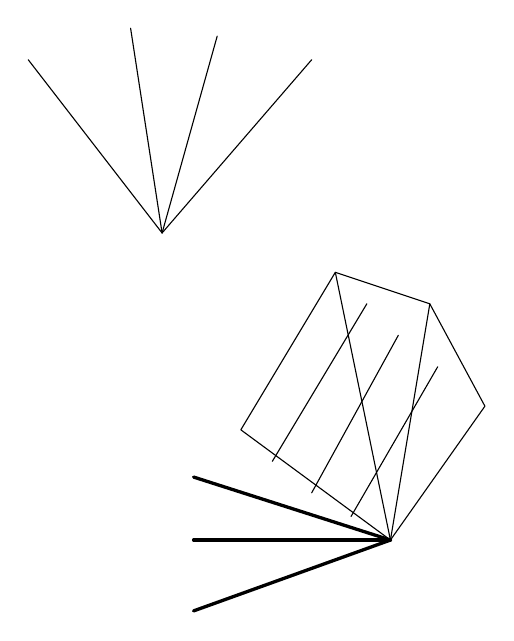
\begin{tikzpicture}[x=1mm,y=1mm,line cap=round,line join=round,font=\scriptsize]
\draw (42,-43) -- (25,-21);
\draw (42,-43) -- (38,-17);
\draw (42,-43) -- (49,-18);
\draw (42,-43) -- (61,-21);
\draw (71,-82) -- (52,-68) -- (64,-48) -- (76,-52) -- (83,-65) -- cycle;
\draw (71,-82) -- (64,-48);
\draw (71,-82) -- (76,-52);
\draw (56,-72) -- (68,-52);
\draw (61,-76) -- (72,-56);
\draw (66,-79) -- (77,-60);
\draw[very thick] (71,-82) -- (46,-74);
\draw[very thick] (71,-82) -- (46,-82);
\draw[very thick] (71,-82) -- (46,-91);
\end{tikzpicture}
\end{document}
